%%%%%%%%%%%%%%%%%%%%%%%%%%%%%%%%%%%%%%%%%
% Programming/Coding Assignment
% LaTeX Template
%
% This template has been downloaded from:
% http://www.latextemplates.com
%
% Original author:
% Ted Pavlic (http://www.tedpavlic.com)
%
% Note:
% The \lipsum[#] commands throughout this template generate dummy text
% to fill the template out. These commands should all be removed when 
% writing assignment content.
%
% This template uses a Perl script as an example snippet of code, most other
% languages are also usable. Configure them in the "CODE INCLUSION 
% CONFIGURATION" section.
%
%%%%%%%%%%%%%%%%%%%%%%%%%%%%%%%%%%%%%%%%%

%----------------------------------------------------------------------------------------
%	PACKAGES AND OTHER DOCUMENT CONFIGURATIONS
%----------------------------------------------------------------------------------------

\documentclass{article}

\usepackage{fancyhdr} % Required for custom headers
\usepackage{lastpage} % Required to determine the last page for the footer
\usepackage{extramarks} % Required for headers and footers
\usepackage[usenames,dvipsnames]{color} % Required for custom colors
\usepackage{graphicx} % Required to insert images
\usepackage{listings} % Required for insertion of code
\usepackage{courier} % Required for the courier font
\usepackage{lipsum} % Used for inserting dummy 'Lorem ipsum' text into the template
\usepackage{url}
% Margins
\topmargin=-0.45in
\evensidemargin=0in
\oddsidemargin=0in
\textwidth=6.5in
\textheight=9.0in
\headsep=0.25in

\linespread{1.1} % Line spacing

% Set up the header and footer
\pagestyle{fancy}
\lhead{\hmwkAuthorName} % Top left header
\chead{\hmwkClass\ (\hmwkClassInstructor\ \hmwkClassTime)} % Top center head
\rhead{\firstxmark} % Top right header
\lfoot{\lastxmark} % Bottom left footer
\cfoot{} % Bottom center footer
\rfoot{Page\ \thepage\ of\ \protect\pageref{LastPage}} % Bottom right footer
\renewcommand\headrulewidth{0.3pt} % Size of the header rule
\renewcommand\footrulewidth{0.4pt} % Size of the footer rule

\setlength\parindent{0pt} % Removes all indentation from paragraphs

%----------------------------------------------------------------------------------------
%	CODE INCLUSION CONFIGURATION
%----------------------------------------------------------------------------------------

\definecolor{MyDarkGreen}{rgb}{0.0,0.4,0.0} % This is the color used for comments
\lstloadlanguages{R} % Load Perl syntax for listings, for a list of other languages supported see: ftp://ftp.tex.ac.uk/tex-archive/macros/latex/contrib/listings/listings.pdf
\lstset{language=R, % Use Perl in this example
        frame=single, % Single frame around code
        basicstyle=\small\ttfamily, % Use small true type font
        breaklines=true,
        keywordstyle=[1]\color{Blue}\bf, % Perl functions bold and blue
        keywordstyle=[2]\color{Purple}, % Perl function arguments purple
        keywordstyle=[3]\color{Blue}\underbar, % Custom functions underlined and blue
        identifierstyle=, % Nothing special about identifiers                                         
        commentstyle=\usefont{T1}{pcr}{m}{sl}\color{MyDarkGreen}\small, % Comments small dark green courier font
        stringstyle=\color{Purple}, % Strings are purple
        showstringspaces=false, % Don't put marks in string spaces
        tabsize=5, % 5 spaces per tab
        %
        % Put standard Perl functions not included in the default language here
        morekeywords={},
        %
        % Put Perl function parameters here
        morekeywords=[2]{on, off, interp},
        %
        % Put user defined functions here
        morekeywords=[3]{test},
       	%
        morecomment=[l][\color{Blue}]{...}, % Line continuation (...) like blue comment
        numbers=left, % Line numbers on left
        firstnumber=1, % Line numbers start with line 1
        numberstyle=\tiny\color{Blue}, % Line numbers are blue and small
        stepnumber=5 % Line numbers go in steps of 5
}

% Creates a new command to include a perl script, the first parameter is the filename of the script (without .pl), the second parameter is the caption
\newcommand{\rscript}[2]{
\begin{itemize}
\item[]\lstinputlisting[caption=#2,label=#1]{#1.R}
\end{itemize}
}

%----------------------------------------------------------------------------------------
%	DOCUMENT STRUCTURE COMMANDS
%	Skip this unless you know what you're doing
%----------------------------------------------------------------------------------------

% Header and footer for when a page split occurs within a problem environment
\newcommand{\enterProblemHeader}[1]{
\nobreak\extramarks{#1}{#1 continued on next page\ldots}\nobreak
\nobreak\extramarks{#1 (continued)}{#1 continued on next page\ldots}\nobreak
}

% Header and footer for when a page split occurs between problem environments
\newcommand{\exitProblemHeader}[1]{
\nobreak\extramarks{#1 (continued)}{#1 continued on next page\ldots}\nobreak
\nobreak\extramarks{#1}{}\nobreak
}

\setcounter{secnumdepth}{0} % Removes default section numbers
\newcounter{homeworkProblemCounter} % Creates a counter to keep track of the number of problems

\newcommand{\homeworkProblemName}{}
\newenvironment{homeworkProblem}[1][Problem \arabic{homeworkProblemCounter}]{ % Makes a new environment called homeworkProblem which takes 1 argument (custom name) but the default is "Problem #"
\stepcounter{homeworkProblemCounter} % Increase counter for number of problems
\renewcommand{\homeworkProblemName}{#1} % Assign \homeworkProblemName the name of the problem
\section{\homeworkProblemName} % Make a section in the document with the custom problem count
\enterProblemHeader{\homeworkProblemName} % Header and footer within the environment
}{
\exitProblemHeader{\homeworkProblemName} % Header and footer after the environment
}

\newcommand{\problemAnswer}[1]{ % Defines the problem answer command with the content as the only argument
\noindent\framebox[\columnwidth][c]{\begin{minipage}{0.98\columnwidth}#1\end{minipage}} % Makes the box around the problem answer and puts the content inside
}

\newcommand{\homeworkSectionName}{}
\newenvironment{homeworkSection}[1]{ % New environment for sections within homework problems, takes 1 argument - the name of the section
\renewcommand{\homeworkSectionName}{#1} % Assign \homeworkSectionName to the name of the section from the environment argument
\subsection{\homeworkSectionName} % Make a subsection with the custom name of the subsection
\enterProblemHeader{\homeworkProblemName\ [\homeworkSectionName]} % Header and footer within the environment
}{
\enterProblemHeader{\homeworkProblemName} % Header and footer after the environment
}

\newcommand{\quotes}[1]{``#1''}
%----------------------------------------------------------------------------------------
%	NAME AND CLASS SECTION
%----------------------------------------------------------------------------------------

\newcommand{\hmwkTitle}{Homework\ \#4} % Assignment title
\newcommand{\hmwkDueDate}{10/2/2017} % Due date
\newcommand{\hmwkClass}{Applied Data Mining} % Course/class
\newcommand{\hmwkClassTime}{Online} % Class/lecture time
\newcommand{\hmwkClassInstructor}{Instructor: Hasan Kurban} % Teacher/lecturer
\newcommand{\hmwkAuthorName}{Keith Hickman} % Your name

%----------------------------------------------------------------------------------------
%	TITLE PAGE
%----------------------------------------------------------------------------------------

\title{
\vspace{2in}
\textmd{\textbf{\hmwkClass:\ \hmwkTitle}}\\
\normalsize\vspace{0.1in}\small{Due\ on\ \hmwkDueDate}\\
\vspace{0.1in}\large{\textit{\hmwkClassInstructor\ }}
\vspace{3in}
}

\author{\textbf{\hmwkAuthorName}}
\date{\today} % Insert date here if you want it to appear below your name

%----------------------------------------------------------------------------------------

\begin{document}

\maketitle

%----------------------------------------------------------------------------------------
%	TABLE OF CONTENTS
%----------------------------------------------------------------------------------------

%\setcounter{tocdepth}{1} % Uncomment this line if you don't want subsections listed in the ToC

%\newpage
%\tableofcontents
\newpage

%%%%%%%%%%%%%%%%%%%%%%%%%%%%%%%%%%
In this homework, you will fit several classifiers to Orange Juice data set (OJ) and compare and discuss the results. The data set can be found in the ISLR package.

\begin{verbatim}
> library(ISLR)
> mydata <- OJ
> names(mydata)
> dim(mydata)
> View(mydata)
             
\end{verbatim}



%%%%%%%%%%%%%%%%%%%%%%%%%%%%%%%%%%

%PROBLEM 1
%%%%%%%%%%%%%%%%%%%%%%%%%%%%%%%%%%
\begin{homeworkProblem}

\subsection{Discussion of Data}
Briefly describe this data set--what is its purpose?  How should it be used? What are the kinds of data it's using?

The orange juice dataset is comparing sales of Minute Made and Cirtus Hill brand orange juices. 
There are 1070 observations of 18 variables. The variables are both discrete and continuous, with most being price-related information such as purchase price and discounts. 
Additionally, the dataset contains purchase location information, whether customers were loyal to a particular brand, and some time series data.
We can use this information to possibly determine what causes customers to purchase one brand versus another - price, loyalty, location, etc... 
My hypothesis is that price will most often dictate the brand being purchased, followed by loyalty. 
 
A complete description of the dataset can be found at https://cran.r-project.org/web/packages/ISLR/ISLR.pdf
 \ldots
\subsection{R Code}
 Using R, show code that answers the following questions:
\begin{enumerate} 
\item How many entries are in the data set?  $\ldots$
There are 1070 observations of 18 variables. 

\rscript{sb11}{Entries in the Dataset}

\item How many unknown or missing data are in the data set?$\ldots$

\rscript{sb12}{Missing and unknown variables}

\item How many Citrus Hill  and  Minute Maid Orange Juice identifiers are there? 
There are 653 Citrus Hill and 417 Minute Maid identifiers. 

\rscript{sb13}{Sample R Script With Highlighting}


\end{enumerate} 
\end{homeworkProblem}


%%%%%%%%%%%%%%%%%%%%%%%%%%%%%%%%%

%PROBLEM 2
%%%%%%%%%%%%%%%%%%%%%%%%%%%%%%%%%%
\begin{homeworkProblem}
Create a training data set containing a random sample of 900 data points and a test set containing the remaining observations.  Name the training data and test data as mydata.training and mydata.testing, respectively.  Place the R code below. You will use mydata.training and mydata.testing to answer the rest of the questions. Thus, create them once and use  mydata.training to train the models (classifiers)  and mydata.testing to test the models. Purchase variable (1st variable in the data) is the response and the other variables are predictors. In addition to answering homework questions, you are encouraged to tune the parameters of the classifiers and test the parameters that are not included in the homework questions.

\subsection{R Code}

\rscript{sb21}{Sample R Script With Highlighting}

\end{homeworkProblem}


%%%%%%%%%%%%%%%%%%%%%%%%%%%%%%%%%

%PROBLEM 3
%%%%%%%%%%%%%%%%%%%%%%%%%%%%%%%%%%
\begin{homeworkProblem}

Fit three decision trees to mydata.training with $se =0,0.5,1$. Visualize the trees in R. Use trees to classify mydata.testing. Calculate a confusion matrix  and accuracy value for each model to evaluate the models. Discuss the results, i.e., which model works best? explain se parameter. How does se parameter affect the results?

The first model with se set to 0 performed the best at classifying whether a given purchase would be made for a given brand.  This model required the lowest level of pruning had the best outcome with the lowest standard error.  Increasing the SE parameter limits the number of pruning steps that can be taken, which requires the model to make more subtle divisions at the root and earlier nodes.  
The model still performed well in testing, but given the most important variable was loyalty, and there was a significant class imbalance in the test dataset, my hypothesis is that this test could be vastly improved with a balanced dataset for both testing and training datasets. 


\subsection{R Code}
Place the R codes below

\begin{enumerate} 

\item  Training code:
 
\rscript{sb31}{Sample R Script With Highlighting}

\item  Testing code: 

\rscript{sb31eval}{Sample R Script With Highlighting}

\end{enumerate}
\subsection{Tree Figures}

 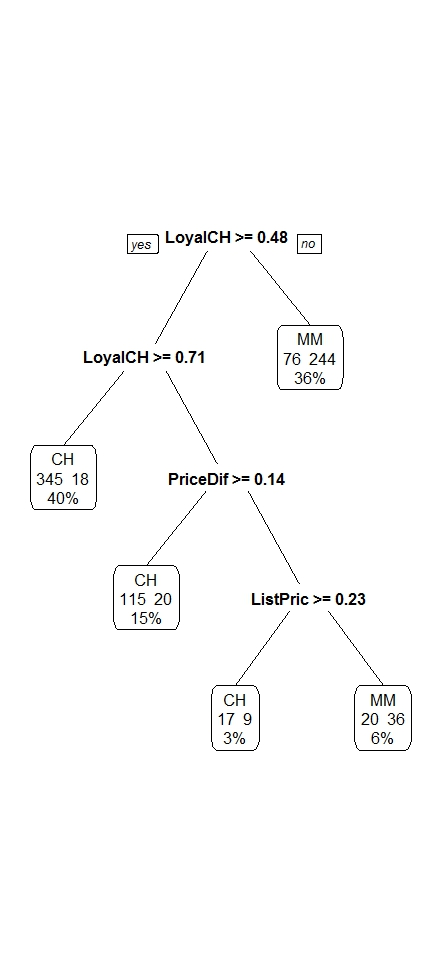
\includegraphics{ct1.jpeg}

 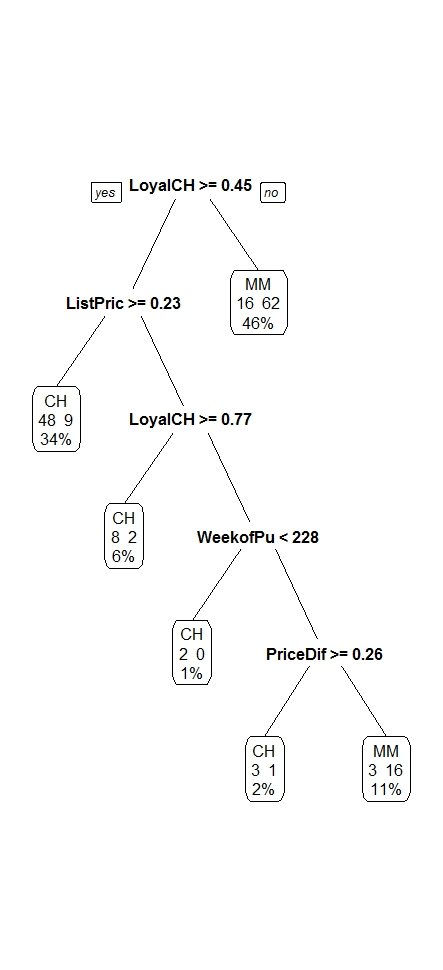
\includegraphics{ct2.jpeg}

 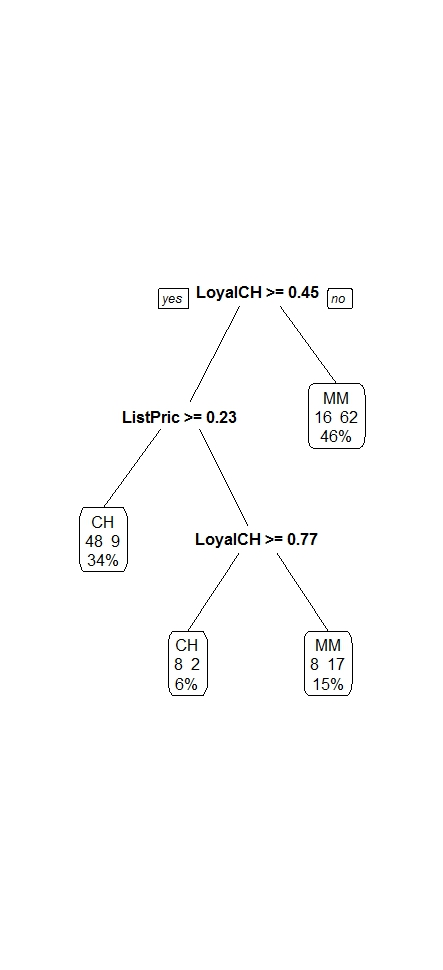
\includegraphics{ct3.jpeg}


\subsection{Results and Discussion}
The Classification Tree performed better than random guessing - about 22-23 percent error rate.  I feel we could improve on this by continuing to engineer features via PCA   \ldots
 
\end{homeworkProblem}

%%%%%%%%%%%%%%%%%%%%%%%%%%%%%%%%%

%PROBLEM 4
%%%%%%%%%%%%%%%%%%%%%%%%%%%%%%%%%%
\begin{homeworkProblem}

In this question, you are asked to train two SVMs over mydata.train and test the models over mydata.testing. (1) Train an SVM with the default settings (radial kernel with constraints violations of cost of 1), (2) Train another SVM with tuning the parameters as follows: cost=$3$, kernel=\quotes{polynomial}, degree=$3$. Create a confusion matrix and calculate the accuracy value for each model. Discuss the results, i.e., Which one performed better? explain the parameters.

The second model performs better by 1 percent. The cost parameter indicates to what degree the model will violate the margins and allow more points across the separation line.


\subsection{R Code}
Place the R codes below

\begin{enumerate} 

\item  Training code:
 
\rscript{sb41train}{Sample R Script With Highlighting}

\item  Testing code: 

\rscript{sb41test}{Sample R Script With Highlighting}

\end{enumerate}

\subsection{Results and Discussion}
The error rate has improved to 12.4 percent, though this could be due to the model overfitting the test data.  I would continue to select various random samples and validate the model does not exhibit any significant changes in error rates. 

\end{homeworkProblem}


%%%%%%%%%%%%%%%%%%%%%%%%%%%%%%%%%

%PROBLEM 5
%%%%%%%%%%%%%%%%%%%%%%%%%%%%%%%%%%
\begin{homeworkProblem}
Fit two Artificial Neural Networks (ANNs) to mydata.training as follows: Set the trace=FALSE and maxit=1000 for both ANNs. The size parameter for the first ANN is $10$ (size=10) and the second one is $50$ (size =50). Test the ANNs over mydata.testing and discuss the results. Which one performed better? explain the parameters? Visualize the ANNs.



\subsection{R Code}
Place the  R codes below

\begin{enumerate} 

\item  Training code:
 
\rscript{sb51}{Sample R Script With Highlighting}

\item  Testing code: 

\rscript{sb}{Sample R Script With Highlighting}

\end{enumerate}
\subsection{ANN Figures}

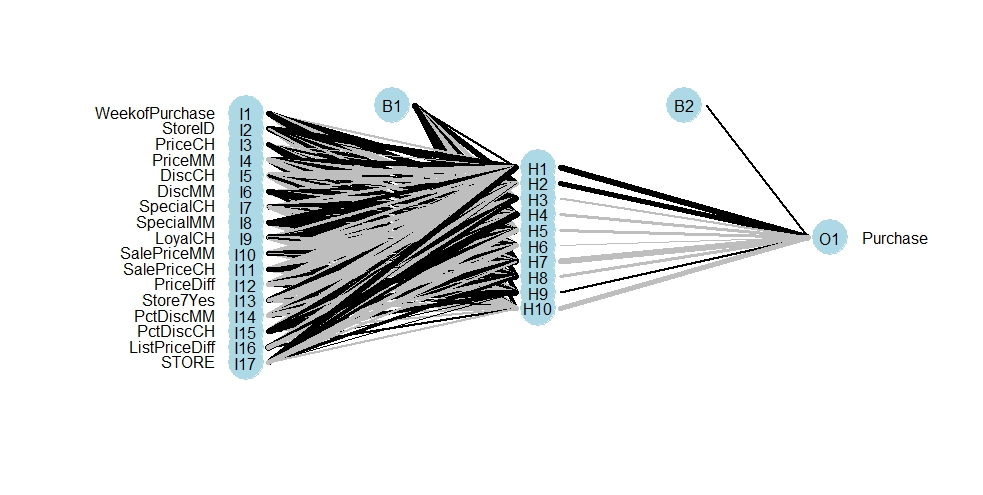
\includegraphics{plotnetn1}

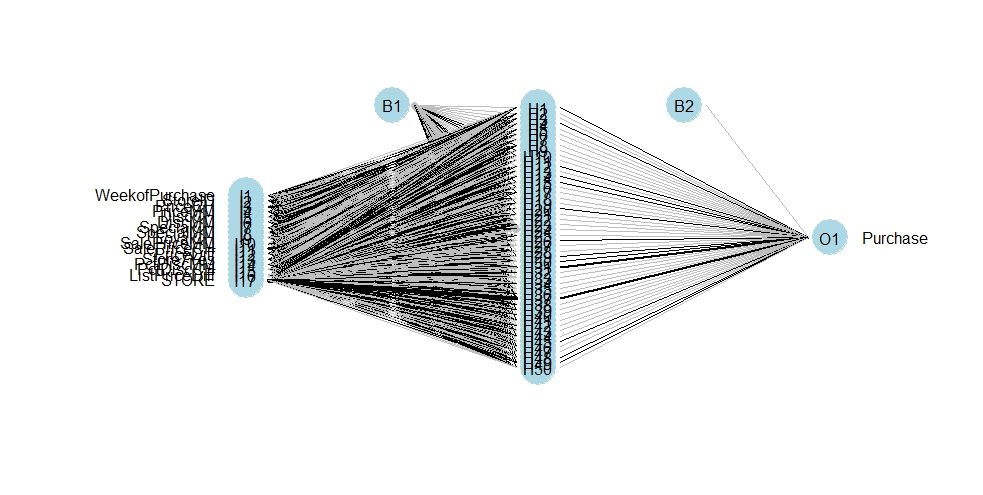
\includegraphics{plotnetn2}

\subsection{Results and Discussion}
The ANNs performed significantly worse on the whole than other models ~ about a 38 percent error rate for both 10 and 50-node models.  Additionally, the models can be somewhat difficult to interpret.
 
\end{homeworkProblem}



%%%%%%%%%%%%%%%%%%%%%%%%%%%%%%%%%

%PROBLEM 6
%%%%%%%%%%%%%%%%%%%%%%%%%%%%%%%%%%
\begin{homeworkProblem}

In this problem, you are asked to train a deep learning model on mydata.training with defaults settings. Test the model over mydata.testing. Calculate the confusion matrix and accuracy value for the model.



\subsection{R Code}
Place the  R code below

\begin{enumerate} 

\item  Training code:
 
\rscript{sb6}{Sample R Script With Highlighting}

\item  Testing code: 

\rscript{sb}{Sample R Script With Highlighting}

\end{enumerate}


\subsection{Results and Discussion}
At first blush, we have several potentially impressive metrics for the DLNN model. An AUC of .91 is suspiciously high. This could be due to overfitting, and additional sampling and testing would be required. An overall error rate of 17 percent is not overly accurate compared to the models we have used thus far.

\begin{verbatim}
MSE:  0.1167534
RMSE:  0.3416919
LogLoss:  0.3641714
Mean Per-Class Error:  0.1624635
AUC:  0.9175802
Gini:  0.8351603
\end{verbatim}
 \ldots
\end{homeworkProblem}


%%%%%%%%%%%%%%%%%%%%%%%%%%%%%%%%%

%PROBLEM 7
%%%%%%%%%%%%%%%%%%%%%%%%%%%%%%%%%%
\begin{homeworkProblem}

Compare the classifiers trained in questions $3,4,5,6$ for Orange Juice data set. Discuss the results.



\subsection{Results and Discussion}
The models used throughout the exercise varied in complexity and ease of interpretation, but were similarly accurate across the board, with the most promising model achieving a mediocre 14 percent error rate.  \ldots
%%%%%%%%%%%%%%%%%%%%%%%%%%%%%%%%%%

\end{homeworkProblem}


\end{document}